\documentclass[a4paper,10pt,conference]{IEEEtran}

\usepackage[noadjust]{cite}
\usepackage{amssymb,amsfonts}
\usepackage{graphicx}
\usepackage{textcomp}
\usepackage{hyperref}
\usepackage{array}
\usepackage{booktabs}
\usepackage[cmex10]{amsmath}
\interdisplaylinepenalty=2500
\usepackage{flushend}

\hypersetup{
  colorlinks=true,
  linkcolor=black,
  citecolor=black,
  urlcolor=blue
}

\def\BibTeX{{\rm B\kern-.05em{\sc i\kern-.025em b}\kern-.08em T\kern-.1667em\lower.7ex\hbox{E}\kern-.125emX}}

\begin{document}

\raggedbottom

\title{Unsupervised Disease Knowledge Mapping from PubMed Abstracts: A Comparative Study of TF-IDF and BioBERT Embeddings with KMeans, HDBSCAN, and Hierarchical Clustering}

\author{\IEEEauthorblockN{Anonymous Author(s)}
\IEEEauthorblockA{Manuscript submitted for double-blind review}}

\maketitle

\begin{abstract}
The exponential growth of biomedical literature, with PubMed exceeding 29 million indexed articles, renders manual synthesis of disease-specific knowledge from abstracts increasingly impractical. Existing computational approaches either require labeled data, impose parametric distributional assumptions, employ general-purpose embeddings that lack domain specificity, or target entity-level extraction rather than unsupervised thematic discovery at the corpus level. To address this gap, we present an unsupervised disease knowledge mapping pipeline that integrates domain-adapted semantic embeddings, nonlinear dimensionality reduction, density-based clustering, and cluster-level term weighting to automatically discover and organize disease research themes from biomedical abstracts. We systematically evaluated two feature extraction strategies—TF-IDF (5,000 features) and BioBERT (768-dimensional contextual embeddings)—combined with UMAP projection and three clustering algorithms (KMeans, HDBSCAN, Hierarchical) across 14,065 PubMed abstracts spanning eight disease categories. TF-IDF with HDBSCAN achieved the highest clustering quality (Silhouette coefficient 0.4786, Davies–Bouldin index 0.6034, NPMI coherence 0.1158), discovering 116 fine-grained topics compared to 5 topics from KMeans-based alternatives. BioBERT with HDBSCAN yielded comparable coherence (NPMI 0.1154, 80 topics), confirming that density-based clustering substantially outperforms parametric approaches for biomedical text organization. Independent clinical validation demonstrated interpretability at two levels: macro-level KMeans produced five clinically meaningful categories (e.g., Cardiovascular \& Metabolic Risk, Neurocognitive Disorders), while micro-level HDBSCAN identified highly specific subtopics with NPMI coherence reaching 0.322 (Ptau Plasma biomarkers). To our knowledge, this is the first study to unify domain-adapted language model embeddings, UMAP-based topological projection, HDBSCAN density clustering, and TF-IDF cluster interpretation into a single disease-targeted pipeline for unsupervised knowledge discovery from biomedical literature.
\end{abstract}

\begin{IEEEkeywords}
Biomedical text mining, unsupervised clustering, BioBERT, TF-IDF, HDBSCAN, UMAP, disease knowledge mapping, PubMed abstracts, topic coherence, natural language processing
\end{IEEEkeywords}

\section{Introduction}

\IEEEPARstart{T}{he} volume of published biomedical research has grown at an accelerating rate over the past two decades. PubMed surpassed 29 million indexed articles by 2019~\cite{ref1}, and disease-specific corpora continue to expand rapidly: neoplasm-related publications alone increased at 42.41\% annually through 2021~\cite{ref13}. This growth creates a fundamental problem for researchers. The knowledge needed to understand a disease, identify research trends, or discover connections across disciplines is distributed across hundreds of thousands of abstracts, each written in specialized terminology that varies by subfield. Manual review at this scale is not feasible, and keyword-based search returns documents matching surface terms rather than organizing them around underlying themes.

Computational approaches to biomedical knowledge extraction have made substantial progress. Domain-adapted language models such as BioBERT~\cite{ref1} have demonstrated that continued pre-training on PubMed abstracts and PMC full-text articles yields significant improvements over general-domain models on named entity recognition, relation extraction, and question answering. Supervised methods have been extended to disease-gene association mining~\cite{ref8}~\cite{ref10}, knowledge graph construction~\cite{ref9}, and document classification~\cite{ref13}, all with strong results where labeled data or predefined ontologies are available. At the same time, unsupervised topic modeling and clustering methods have evolved from bag-of-words models such as Latent Dirichlet Allocation (LDA) toward approaches that incorporate contextual embeddings from transformer architectures~\cite{ref15}~\cite{ref17}.

Despite these advances, three limitations persist in the existing literature. First, most biomedical NLP evaluations focus on supervised tasks: entity recognition, relation extraction, and document classification~\cite{ref2}~\cite{ref3}~\cite{ref4}~\cite{ref5}~\cite{ref6}. Unsupervised discovery of thematic structure at the corpus level, where no labels exist to guide the analysis, has received comparatively less attention. Second, among the clustering and topic modeling studies that do exist~\cite{ref15}~\cite{ref16}~\cite{ref17}, the embedding stage typically relies on either sparse frequency-based features (TF-IDF, bag-of-words) or general-purpose sentence transformers, neither of which fully exploits the domain-specific representational capacity of biomedical language models. Third, existing clustering frameworks either impose parametric assumptions about cluster distributions, as Gaussian Mixture Models (GMM) and KMeans do, or produce topic representations that require manual inspection without automated labeling~\cite{ref17}. No prior study has, to our knowledge, integrated domain-adapted embeddings, nonlinear dimensionality reduction, density-based clustering, and cluster-level term weighting into a single unsupervised pipeline for disease-specific knowledge discovery from PubMed abstracts.

We address this gap by designing and systematically evaluating a modular unsupervised pipeline for disease knowledge mapping. The pipeline comprises four stages: (1) feature extraction via either TF-IDF vectorization (5,000 features) or BioBERT 768-dimensional contextual embeddings; (2) nonlinear dimensionality reduction using Uniform Manifold Approximation and Projection (UMAP) with cosine distance; (3) clustering via three algorithms representing different inductive biases: KMeans (partition-based), HDBSCAN (density-based), and agglomerative hierarchical clustering (connectivity-based); and (4) automated topic interpretation using cluster-level TF-IDF keyword extraction. The pipeline is evaluated across 14,065 PubMed abstracts collected from eight disease categories (diabetes, cancer, cardiovascular disease, neurological disorders, stroke, hypertension, Alzheimer's, and Parkinson's) using the NCBI E-utilities API.

The experimental design compares all six configurations formed by crossing two embedding methods with three clustering algorithms. We assess clustering quality using three complementary metrics: Silhouette coefficient (cluster separation), Davies--Bouldin index (intra-cluster compactness), and Normalized Pointwise Mutual Information (NPMI) coherence (topic interpretability). Clinical interpretability is validated at two granularity levels: macro-level categorization through KMeans clusters and micro-level topic discovery through HDBSCAN clusters.

Our main findings are as follows. The TF-IDF with HDBSCAN configuration achieves the highest overall clustering quality (Silhouette~0.4786, Davies--Bouldin~0.6034, NPMI~0.1158), discovering 116 fine-grained topics. BioBERT with HDBSCAN yields comparable topic coherence (NPMI~0.1154, 80 topics), confirming that density-based clustering substantially outperforms parametric approaches regardless of the embedding method. The parametric algorithms (KMeans, Hierarchical) are constrained to exactly five topics by the Elbow method and produce consistently lower coherence scores (NPMI~0.06--0.08). The macro-level KMeans clusters map to five clinically meaningful categories: Cardiovascular \& Metabolic Risk, Preclinical Molecular Biology, Oncology \& Case Studies, Clinical Outcomes \& Mortality, and Neurocognitive Disorders. The micro-level HDBSCAN topics include highly specific subtopics with NPMI coherence reaching 0.322 for Ptau Plasma biomarkers and 0.282 for Syn Disease aggregation pathways, demonstrating that the density-based approach captures both broad clinical categories and narrow specialized research themes within a single corpus.

The contributions of this work are threefold. (1) We present the first unified unsupervised pipeline that integrates BioBERT semantic embeddings, UMAP topological projection, HDBSCAN density clustering, and cluster-level TF-IDF keyword extraction for disease knowledge mapping from PubMed abstracts. (2) We provide a systematic comparative evaluation of two embedding strategies and three clustering algorithms across six configurations using three complementary metrics on a multi-disease corpus of 14,065 abstracts. (3) We demonstrate clinical interpretability at two granularity levels with independently validated topic coherence scores, establishing that density-based clustering with frequency-based features is competitive with contextual embeddings for unsupervised topic discovery in biomedical text.

The remainder of this paper is organized as follows. Section~II reviews related work in biomedical language models, literature mining, unsupervised clustering, and embedding visualization. Section~III describes the dataset collection, preprocessing pipeline, and methodological details of all six experimental configurations. Section~IV presents the quantitative results and clinical validation at both macro and micro levels. Section~V discusses the implications, limitations, and directions for future work. Section~VI concludes the paper.

\section{Related Work}

The number of biomedical publications is increasing every year. PubMed had over 29 million indexed articles by 2019~\cite{ref1}, and disease-specific fields keep growing, with neoplasm-related publications increasing at 42.41\% annually through 2021~\cite{ref13}. Keeping up with that volume manually is no longer realistic. There is real scientific knowledge inside those abstracts, but extracting it in an organized, usable form requires computational tools that go beyond keyword search. Researchers have worked on this from four directions: building biomedical language models, mining abstracts for disease knowledge, grouping documents without supervision, and visualizing semantic structure. Each of these directions has produced meaningful results. Yet these directions have rarely been integrated with one another. To the best of our knowledge, few existing studies have integrated all four into a single, disease-specific knowledge mapping pipeline from biomedical literature. 

\subsection{Biomedical Language Models for Biomedical NLP}

Biomedical text does not behave like general text. The vocabulary is specialized, terms carry context-dependent meaning, and the same concept can appear in dozens of different surface forms across papers. Early NLP systems handled this with Conditional Random Fields (CRF) and Support Vector Machines (SVM), both of which required heavy hand-crafted features and broke down when terms were rare or ambiguous~\cite{ref2}. BiLSTM-CRF networks improved sequence labeling. Capturing the full contextual meaning of a biomedical sentence, though, was still beyond what those architectures could do~\cite{ref2}. BERT brought a better foundation through self-attention across full sequences. The problem was that it was trained only on Wikipedia and BooksCorpus. That is general text. Biomedical writing is different, and the mismatch had a measurable effect on performance. 

Lee et al.~\cite{ref1} addressed this directly by continuing BERT pre-training on PubMed abstracts and PMC full-text articles, producing BioBERT. Compared to general BERT, BioBERT gained 0.62\% F1 on named entity recognition, 2.80\% F1 on relation extraction, and 12.24\% MRR on question answering. The takeaway from these results is plain: a model understands the text it was trained on, and biomedical text needs a model trained on biomedical data. Peng et al.~\cite{ref3} confirmed this across a wider range of tasks through the BLUE benchmark, which evaluated models on ten biomedical and clinical NLP corpora. Models pre-trained on PubMed and MIMIC-III ranked highest across every task type, with clinical text showing the largest gains. Both studies point to the same conclusion: domain mismatch between pre-training data and target text is not a minor issue. It carries a real cost on downstream performance. 

Beyond what a model is trained on, how it is trained also matters. Peng et al.~\cite{ref4} applied multi-task learning across several biomedical NLP objectives and measured gains of 2.0\% and 1.3\% in biomedical and clinical settings over single-task models. Training across related tasks together produces representations that generalize better than training for one task alone. Alrowili and Vijay-Shanker~\cite{ref5} showed through the BioM-Transformers family that careful design choices, including model size, training objective, and corpus selection, can reach state-of-the-art results without increasing computational costs. Together, these studies show that embedding quality depends on how a model is built and trained, not just on the volume of data it sees. 

Vithanage et al.~\cite{ref6} compared 18 contextual embedding models, including ELMo, BERT, BioBERT, BlueBERT, Clinical BioBERT, GPT-3, and others, across classification, NER, and question answering tasks drawn from PubMed and clinical EHR data. BioBERT ranked highest on general biomedical text across all task types. That makes it the most empirically supported choice for embedding PubMed abstracts. Kumar and Basu~\cite{ref2} took BioBERT further with AdaBioBERT, adding an adaptive loss function to improve recognition of rare and contextually sensitive biomedical terms of the kind that standard NER models tend to misclassify. 

Sharaf and Anoop~\cite{ref7} looked at what happens when BioBERT is used in real clinical systems. Performance improved in areas like decision support and information retrieval. Practical barriers emerged too: patient data privacy, bias in training corpora, and the overhead of domain-specific adaptation. These concerns do not apply to the present study. The analysis uses only publicly available PubMed abstracts, involves no patient records, and requires no task-specific fine-tuning. 

\subsection{Biomedical Literature Mining and Disease Knowledge Discovery}

The idea of extracting disease knowledge automatically from biomedical literature is not new. The oldest and most common approach is co-occurrence mining: if a disease term and a gene symbol appear frequently together in the same abstract, the system infers a relationship. Grissa et al.~\cite{ref8} built DISEASES 2.0 on this principle, a continuously updated database that mines PubMed for disease-gene links and integrates results with GWAS evidence and curated data sources. When full-text articles were added alongside abstracts, mined associations increased nine-fold. That shows how much signal even abstract-level text carries. Still, co-occurrence mining only produces flat pairwise lists. It tells you nothing about how topics in the literature are organized, which research directions dominate, or how disease themes relate at a document level. 

Xu et al.~\cite{ref9} built something structurally richer. Their PubMed knowledge graph (PKG), drawn from 29 million abstracts, used BioBERT for bio-entity extraction, which outperformed prior tools by 0.51\% F1, and integrated author networks, funding, and institutional affiliations alongside biological entities. It is a useful resource for studying how biomedical knowledge flows across institutions and disciplines. Its organization, however, centers on entity-level links. The thematic distribution of disease research, including which topics are prominent, which are marginal, and how they relate, is not what it is designed to capture. Diaz Gonzalez et al.~\cite{ref10} applied the same logic to germline genetics, using BioBERT to construct SimpleGermKG with 297 genes, 130 diseases, and over 46,000 relational triples, with ontology-based normalization to standardize term variation. Like the PKG, its output is organized around fixed entity types. 

Research themes outside the predefined schema simply do not appear. Li et al.~\cite{ref11} moved closer to semantic territory with LORE, an unsupervised framework that reads PubMed abstracts as collections of verifiable relational statements and represents gene-disease pairs as embeddings in Euclidean space. Tested across 2,097 diseases, LORE reached 90\% mean average precision for pathogenic gene identification. A 2D UMAP projection of the embedding space also showed that pathogenic disease-gene pairs form a visually distinct region, which suggests that semantic embeddings of biomedical text can carry geometric structure with biological meaning. LORE is the closest prior work in aim to the present study. Even so, its output is a ranked gene list. The abstract itself, including its research context, disease framing, and scientific narrative, is not what the system is analyzing. 

Supervised extraction methods have achieved strong results, yet they require labeled data and predefined schemas. Zhang et al.~\cite{ref12} converted syntactically complex biomedical sentences into structured semantic graphs using Abstract Meaning Representation (AMR) and enriched those graphs with external ontological knowledge. On the GENIA 2011 benchmark, this approach gained 1.8\% from AMR and 3.0\% from knowledge enrichment, with further validation on COVID-19 literature. The system performs well for the entity types and events it was trained to find. Anything outside those predefined categories goes undetected, regardless of how frequently it appears in the data. Masoumi et al.~\cite{ref13} illustrated the same boundary at classification scale: BioBERT classifiers trained on 12,817 PubMed abstracts categorized documents into predefined medical fields with 76\%--86\% micro F1. The system works within its defined taxonomy and nowhere else. 

Chuang et al.~\cite{ref14} took a different direction with DiscoverPath, a NER-based retrieval system that builds entity relationship graphs from biomedical abstracts to help researchers navigate cross-disciplinary vocabulary. It solves a real search problem. Search and discovery are not the same thing, however. DiscoverPath helps a researcher find papers they already know to look for. There are things that a researcher does not know to look for. These things remain out of reach for the researcher. The researcher just does not know where to find these themes. So, these themes are out of reach for the researcher. 

\subsection{Unsupervised Clustering and Topic Modeling in Biomedical Text}

When we do not have any labels, unsupervised clustering is the way we find structure in Biomedical Text. We use topic models like LDA and NMF to do this. These topic models take each document. Turn it into a bag of words. When they do this, they get rid of all the information about how the terms in the Biomedical Text are related to each other. They also lose the information about how the meaning of the terms in the Biomedical Text changes when the context changes. They forget about the order of the words in the sentences of the Biomedical Text~\cite{ref15}. TF-IDF vectors have the same problem: they count word frequency, not word meaning. Clusters produced this way reflect surface vocabulary overlap, not conceptual organization. In biomedical text, where researchers describing the same biological mechanism often use entirely different terminology depending on the subfield, this is a real and significant problem. 

Contextual embeddings from transformer models changed what was possible here. In a PubMed clustering experiment, Davagdorj et al.~\cite{ref15} evaluated this by running GMM against K-Means, DBSCAN, and agglomerative techniques and substituting BioBERT embeddings for TF-IDF vectors. In all three evaluation metrics: the Davies-Bouldin score (1.6849), the adjusted rand index (0.4478), and the silhouette coefficient (0.3765), the BioBERT-GMM combo came in first. When the representation carries semantic content, the clusters reflect it. GMM's limitation, however, is that it requires the analyst to fix the number of clusters in advance and assumes each cluster takes an approximately Gaussian shape. Biomedical research themes do not follow that distribution. They vary widely in size, overlap in unpredictable ways, and have no reason to be normally distributed. 

AbdelAziz et al.~\cite{ref16} combined BERT embeddings with topic modeling and hierarchical clustering for extractive summarization of 200 biomedical papers, reaching ROUGE-1 of 0.4838 with expert completeness ratings averaging 4.10. The sequential structure of their approach, which involves embedding, clustering, and keyword extraction, resembles the kind of pipeline used for document-level knowledge organization. Summarizing individual documents and mapping themes across a corpus are different problems, and AbdelAziz et al. are solving the former. 

Grootendorst~\cite{ref17} introduced BERTopic, the most methodologically relevant prior work in this space. BERTopic generates document embeddings from a transformer model, clusters them with HDBSCAN, and labels each cluster using a class-based TF-IDF procedure called c-TF-IDF, which weights terms by their importance within a cluster rather than across the whole corpus. This is an important design insight. A term like ``metformin'' may appear in thousands of abstracts. Its elevated frequency within one specific cluster, however, identifies that cluster as diabetes-related far more precisely than any global frequency measure could. BERTopic performs well against LDA and other topic models. Where it falls short for the present purpose is in the embedding stage: BERTopic uses general sentence-transformer models, not biomedical-domain ones. The representational depth that BioBERT gains from PubMed and PMC pre-training is simply not part of its design. 

Munoz-Farre et al.~\cite{ref18} offered a useful perspective from clinical data: transformer embeddings combined with time-series clustering stratified UK Biobank participants with type 2 diabetes into distinct patient subgroups with different aetiological and prognostic profiles. The input is structured EHR data rather than text. The core finding still carries across: deep embeddings, when organized through density-based clustering, can surface disease-specific structure without any labeled supervision. 

\subsection{Visualization and Knowledge Mapping of Biomedical Embeddings}

High-dimensional embeddings are not interpretable on their own. Dimensionality reduction is needed to make the structure they encode visible and analyzable. Oubenali et al.~\cite{ref19} reviewed 30 studies on visualization methods for biomedical word embeddings across PubMed, MedRxiv, and arXiv. UMAP and t-SNE came up most often across the reviewed studies. What the review also noted was that no consistent guidelines exist for when to use which method or how to interpret the projections produced. Studies use visualization interchangeably for exploration, evaluation, and presentation, often without clarifying which purpose is being served. In most cases, visualization is applied after conclusions have already been drawn by other means. When that happens, the ability of the visualization to reveal a new structure that was not already known goes mostly unused. 

UMAP has specific properties that make it well-suited to this kind of analysis. Grounded in Riemannian geometry and algebraic topology, it preserves both local neighborhood structure and global data topology more faithfully than t-SNE, while scaling efficiently to large datasets~\cite{ref19}. Panesar~\cite{ref20} provided evidence that BioBERT embeddings are particularly well-matched to UMAP projection: contextual representations from BioBERT capture relational knowledge between biomedical concepts more accurately than static models like Word2Vec, especially for functional and mechanistic relationships that describe disease processes. In 2D UMAP projections of these representations, spatial proximity reflects genuine semantic relatedness rather than surface-level co-occurrence. 

Li et al.~\cite{ref11} showed what this looks like in practice. When disease-gene embeddings were projected using UMAP and colored by ClinVar pathogenicity labels, pathogenic associations formed a geometrically distinct region with a smooth gradient across the embedding space. That kind of structure simply cannot be seen in a table or a ranked list. Xu et al.~\cite{ref9}, and Chuang et al.~\cite{ref14} both used visualization in their respective systems, primarily to display graph-based entity relationships: one focusing on scholarly connection networks in PubMed, and the other on cross-disciplinary terminology navigation. Graph topology and semantic embedding geometry are different things, serving different purposes. Neither system attempts to map how disease research themes are distributed across a document corpus. 

\subsection{Research Gap and Motivation}

Across the four areas reviewed above, the pattern is consistent. Biomedical language models produce strong, domain-aware embeddings~\cite{ref1}~\cite{ref2}~\cite{ref3}~\cite{ref4}~\cite{ref5}~\cite{ref6}~\cite{ref7}, yet evaluations have focused almost entirely on supervised tasks. Literature mining builds entity graphs and association databases at an impressive scale~\cite{ref8}~\cite{ref9}~\cite{ref10}~\cite{ref11}~\cite{ref12}~\cite{ref13}~\cite{ref14}. Those outputs, however, are organized around predefined schemas, and the data-driven thematic structure of a disease corpus is simply not what these systems are built to reveal. Clustering and topic modeling have adopted contextual embeddings~\cite{ref15}~\cite{ref16}~\cite{ref17}~\cite{ref18}. The existing frameworks, at the same time, either impose parametric assumptions that biomedical research themes do not satisfy, use general-purpose embedding models that miss the advantages of biomedical pre-training, or target document summarization rather than corpus-level theme discovery. Visualization tools have been applied to biomedical embedding spaces~\cite{ref11}~\cite{ref19}~\cite{ref20}, mostly as a post-hoc display layer rather than as an integrated analytical stage in the discovery process. 

To the best of our knowledge, no existing study has combined BioBERT-based semantic embeddings, UMAP dimensionality reduction, HDBSCAN density clustering, and TF-IDF cluster keyword extraction into a unified, disease-targeted pipeline for unsupervised knowledge discovery from PubMed abstracts. The individual components have each been studied. Domain-adapted language models, density-based clustering, cluster-level keyword interpretation, and UMAP-based projection all exist and have been validated in relevant contexts. What has not been done is combining them specifically for the purpose of mapping disease knowledge from biomedical literature without labeled data. That gap is what this study addresses.

\section{Methodology}

Fig.~\ref{fig:pipeline} presents the complete pipeline architecture, comprising eight sequential stages: data acquisition, text preprocessing, feature extraction (TF-IDF or BioBERT), pseudo-class centroid analysis, UMAP dimensionality reduction, clustering (KMeans, HDBSCAN, and hierarchical), topic and keyword extraction, and automated disease knowledge mapping. Each stage is described in detail in the following subsections.

\begin{figure}[t]
\centering
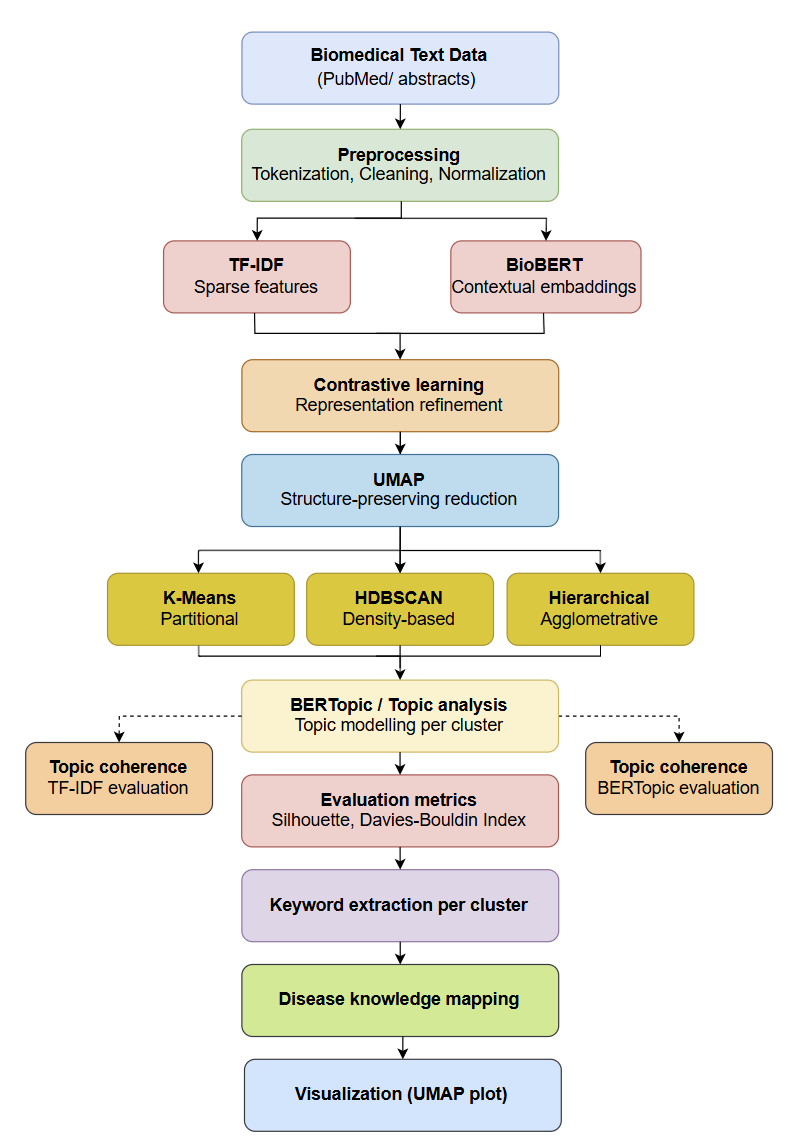
\includegraphics[width=\columnwidth]{Manuscript_Results/Complete_pipeline_architecture.png}
\caption{Pipeline architecture for unsupervised disease knowledge mapping from PubMed abstracts. The modular design supports interchangeability of the feature extraction and clustering components, yielding six experimental configurations.}
\label{fig:pipeline}
\end{figure}

\subsection{Dataset Description}

The corpus was constructed by querying the NCBI E-utilities API with Entrez.email = "noreply.studyhubteam@gmail.com" using eight disease-specific search terms: ``diabetes mellitus,'' ``cancer neoplasm,'' ``cardiovascular disease,'' ``neurological disorders,'' ``stroke cerebrovascular,'' ``hypertension blood pressure,'' ``Alzheimer disease dementia,'' and ``Parkinson disease.'' For each query, up to 2,000 PubMed identifiers (PMIDs) were retrieved using Entrez.esearch with history server support (usehistory="y"). Abstracts were fetched in batches of 200 via Entrez.efetch in XML format with a 0.4-second delay between batches to comply with NCBI rate limits of three requests per second. Cross-query PMID deduplication ensured that each abstract appeared only once, with its first associated disease label retained. Abstracts with empty content were removed, and a second pass eliminated duplicate abstract text.

The final dataset contains 14,065 records across eight disease categories with the following distribution: cancer neoplasm (1,951), diabetes mellitus (1,922), stroke cerebrovascular (1,880), Alzheimer disease dementia (1,753), hypertension blood pressure (1,747), cardiovascular disease (1,722), neurological disorders (1,586), and Parkinson disease (1,504). Each record comprises a PMID, title, abstract text, and disease category label. The labels were used only for descriptive analysis of cluster composition, not for supervised training.

\subsection{Text Preprocessing}

All abstracts underwent the same preprocessing pipeline in both the TF-IDF and BioBERT configurations. For each abstract, the text was lowercased and non-alphabetic characters were removed using the regular expression [\textasciicircum a-zA-Z\textbackslash s]. Tokens were extracted via NLTK's word\_tokenize, English stop words were removed using NLTK's standard stop word list, and tokens with length two characters or fewer were discarded. Documents that reduced to empty strings after preprocessing were removed, reducing the corpus from 14,065 to 14,064 documents.

\subsection{Feature Extraction}

The pipeline evaluates two fundamentally different approaches to document representation.

\subsubsection{TF-IDF Vectorization}

The term frequency--inverse document frequency (TF-IDF) scheme transforms each document into a sparse vector weighted by term salience. The term frequency $\text{TF}(t,d)$ measures the occurrence count $f_{t,d}$ of term $t$ in document $d$ normalized by the total terms in that document:

\begin{equation}
\text{TF}(t,d) = \frac{f_{t,d}}{\sum_{k} f_{k,d}}
\end{equation}

The inverse document frequency $\text{IDF}(t)$ down-weights terms that appear in many documents:

\begin{equation}
\text{IDF}(t) = \log \frac{N}{1 + n_t}
\end{equation}

where $N$ is the total number of documents and $n_t$ is the number of documents containing term $t$. The combined TF-IDF weight is:

\begin{equation}
\text{TFIDF}(t,d) = \text{TF}(t,d) \times \text{IDF}(t)
\end{equation}

We used sklearn.feature\_extraction.text.TfidfVectorizer with parameters max\_features=5000, min\_df=5, max\_df=0.9, and stop\_words='english', producing a sparse document--term matrix of shape $14064 \times 5000$. The matrix was L2-normalized row-wise using sklearn.preprocessing.normalize(norm='l2') to ensure unit-length document vectors.

\subsubsection{BioBERT Contextual Embeddings}

For the semantic embedding configuration, we used the pretrained BioBERT model (dmis-lab/biobert-v1.1})~\cite{ref1}, a bidirectional transformer encoder initialized from BERT-base and further pretrained on PubMed abstracts and PMC full-text articles. The model produces 768-dimensional contextual representations that capture the meaning of each token in its surrounding context.

Each preprocessed abstract was tokenized using the BioBERT WordPiece tokenizer with a maximum sequence length of 128 tokens, applying padding and truncation as needed. The model was run in evaluation mode (model.eval()}) with gradient tracking disabled. Abstracts were processed in batches of 32. For each document, the document-level embedding $\mathbf{E}_d$ was obtained by mean pooling the last hidden state over the sequence dimension, weighting by the attention mask to exclude padding tokens:

\begin{equation}
\mathbf{E}_d = \frac{\sum_{l=1}^{L} \mathbf{h}_l \cdot m_l}{\sum_{l=1}^{L} m_l}
\end{equation}

where $\mathbf{h}_l \in \mathbb{R}^{768}$ is the last hidden state at position $l$, $m_l \in \{0,1\}$ is the attention mask value at position $l$, and $L$ is the sequence length. The resulting 768-dimensional vectors were L2-normalized identically to the TF-IDF pipeline. BioBERT embedding extraction for the full 14,064-document corpus required approximately 35 minutes on CPU; GPU acceleration is supported when available via \text{torch.device('cuda')}.

\subsection{Pseudo-Class Centroid Analysis}

After feature extraction, we performed an intermediate diagnostic step to assess the semantic structure of the embedding space. KMeans clustering with $K=10$ (random\_state=42}, n\_init=5}) was applied to the normalized feature matrix to produce pseudo-class labels. For each of the ten pseudo-classes, the centroid vector was computed as the mean of all document embeddings assigned to that class. The pairwise cosine similarity matrix of the ten centroids was then calculated. This step, labeled contrastive learning in the pipeline, is not a training objective but an exploratory diagnostic that provides a snapshot of inter-concept separation before the full clustering pipeline. Higher centroid cosine similarity indicates less separable pseudo-classes, and vice versa.

\subsection{Dimensionality Reduction with UMAP}

Uniform Manifold Approximation and Projection (UMAP) was applied to reduce the high-dimensional normalized feature matrices to two dimensions for clustering and visualization. UMAP constructs a fuzzy simplicial set representation of the high-dimensional data and optimizes a low-dimensional embedding that preserves topological structure. The optimization minimizes the cross-entropy between the high-dimensional and low-dimensional graph representations:

\begin{equation}
\min_{Y} \sum_{i,j} w_{ij} \| \mathbf{y}_i - \mathbf{y}_j \|^2
\end{equation}

where $w_{ij}$ is the weight encoding the similarity between points $i$ and $j$ in the high-dimensional space, and $\mathbf{y}_i, \mathbf{y}_j \in \mathbb{R}^2$ are their low-dimensional embeddings.

We used the following parameters consistent across both pipelines: n\_components=2}, n\_neighbors=15}, min\_dist=0.1}, metric='cosine'}, and random\_state=42}. The cosine metric is appropriate for L2-normalized vectors, as cosine distance corresponds to Euclidean distance on the unit hypersphere. The output coordinates (UMAP1}, UMAP2}) serve as the input to all downstream clustering algorithms.

\subsection{Clustering Methods}

The optimal number of clusters for partition-based and connectivity-based methods was determined automatically using the Elbow method applied to the UMAP 2D embeddings. KMeans was fitted for $k$ from 2 to 15 (random\_state=42}, n\_init=10}), and the optimal $k$ was identified as the point maximizing perpendicular distance from the line connecting the first and last points of the inertia curve:

\begin{equation}
d_k = \frac{\| (\mathbf{p}_2 - \mathbf{p}_1) \times (\mathbf{p}_1 - \mathbf{p}_k) \|}{\| \mathbf{p}_2 - \mathbf{p}_1 \|}
\end{equation}

where $\mathbf{p}_1 = (2, I_2)$, $\mathbf{p}_2 = (15, I_{15})$, and $\mathbf{p}_k = (k, I_k)$, with $I_k$ denoting the inertia at $k$. This procedure yielded an optimal $K = 5$ for both the TF-IDF and BioBERT pipelines.

Three clustering algorithms with distinct inductive biases were applied to the UMAP embeddings of each pipeline.

\subsubsection{KMeans Clustering}

KMeans partitions the data into $K$ clusters by minimizing the within-cluster sum of squared distances:

\begin{equation}
J = \sum_{i=1}^{K} \sum_{\mathbf{x} \in C_i} \| \mathbf{x} - \boldsymbol{\mu}_i \|^2
\end{equation}

where $C_i$ is the $i$-th cluster and $\boldsymbol{\mu}_i$ is its centroid. We used $K=5$ with random\_state=42} and n\_init=20} to reduce sensitivity to initialization.

\subsubsection{HDBSCAN Clustering}

Hierarchical Density-Based Spatial Clustering of Applications with Noise (HDBSCAN) identifies clusters as regions of high density separated by low-density regions. It constructs a mutual-reachability-distance-based minimum spanning tree, builds a condensed hierarchy of candidate clusters, and selects the most persistent clusters using a stability criterion. Points in low-density regions are labeled as noise (label --1), enabling the algorithm to avoid forcing every observation into a cluster. We used min\_cluster\_size=30}, min\_samples=5}, and metric='euclidean'}. Unlike KMeans and hierarchical clustering, HDBSCAN determines the number of clusters automatically from the data's density structure; in our experiments it discovered 116 clusters for the TF-IDF pipeline and 80 clusters for the BioBERT pipeline.

\subsubsection{Hierarchical Clustering}

Agglomerative hierarchical clustering with Ward's linkage was used as a connectivity-based baseline. The algorithm proceeds by initially placing each document in its own singleton cluster and then iteratively merging the pair of clusters that minimizes the increase in total within-cluster variance. We used $K=5$ with linkage='ward'} to match the KMeans configuration.

\subsection{Topic and Keyword Extraction}

For each clustering solution, topics were derived using two complementary approaches. First, a count-based approach (CountVectorizer} with max\_features=500}, min\_df=2}, stop\_words='english'}) was applied within each cluster to extract the 15 most frequent terms, providing a raw frequency-based topic signature. Second, a TF-IDF-based keyword extraction used TfidfVectorizer} (max\_features=200}, min\_df=1}, stop\_words='english'}) fitted per cluster independently, with the 15 terms having the highest mean TF-IDF score serving as discriminative keywords. These cluster-level TF-IDF scores identify terms that are distinctive within a cluster relative to its own document population, complementing the global frequency view.

\subsection{Disease Knowledge Mapping}

Clusters were automatically mapped to interpretable disease topics by extracting the two highest-scoring terms from a cluster-specific TF-IDF vectorizer (max\_features=100}, stop\_words='english'}), joining them with ``\&'', and converting to title case. For example, a cluster whose top two terms were ``ptau'' and ``plasma'' received the label ``Ptau \& Plasma''. Noise points identified by HDBSCAN (label --1) were excluded from mapping and labeled ``Noise.'' This procedure provides a zero-shot, data-driven semantic label for every cluster without requiring manual annotation.

\subsection{Evaluation Metrics}

Clustering quality was assessed using two intrinsic metrics. The Silhouette coefficient measures how similar a point is to its own cluster compared to other clusters:

\begin{equation}
S = \frac{1}{N} \sum_{i=1}^{N} \frac{b(i) - a(i)}{\max(a(i), b(i))}
\end{equation}

where $a(i)$ is the mean intra-cluster distance for point $i$ and $b(i)$ is the mean distance to the nearest neighboring cluster. Scores range from $-1$ (incorrect clustering) through $0$ (overlapping clusters) to $+1$ (well-separated clusters).

The Davies--Bouldin index evaluates intra-cluster compactness relative to inter-cluster separation:

\begin{equation}
\text{DB} = \frac{1}{K} \sum_{i=1}^{K} \max_{j \neq i} \frac{\sigma_i + \sigma_j}{d(\mathbf{c}_i, \mathbf{c}_j)}
\end{equation}

where $\sigma_i$ is the average distance of points in cluster $i$ to its centroid $\mathbf{c}_i$, and $d(\mathbf{c}_i, \mathbf{c}_j)$ is the distance between cluster centroids. Lower values indicate more compact and better-separated clusters. For HDBSCAN, both metrics were computed exclusively on non-noise points (labels $\neq -1$) to avoid confounding density-based outlier detection with cluster quality assessment.

Topic interpretability was evaluated using Normalized Pointwise Mutual Information (NPMI) coherence, computed independently using the UCI coherence formula. For each cluster, the top 10 terms by TF-IDF score were extracted, and NPMI was computed over all term pairs using a binary document--term matrix constructed from the full corpus (CountVectorizer} with min\_df=5}, max\_df=0.95}, binary=True}, stop\_words='english'}; vocabulary size 16,286). The NPMI for a pair of terms $(w_i, w_j)$ is defined as:

\begin{equation}
\text{NPMI}(w_i, w_j) = \frac{\log \frac{P(w_i, w_j)}{P(w_i) P(w_j)}}{-\log P(w_i, w_j)}
\end{equation}

where $P(w_i)$ is the document fraction containing $w_i$, and $P(w_i, w_j)$ is the fraction of documents containing both $w_i$ and $w_j$. Per-topic NPMI is the mean across all unique term pairs in the topic's top-10 term list. Scores range from $-1$ (perfectly anti-correlated) to $+1$ (perfectly correlated), with positive values indicating semantically coherent topics.

\section{Results}

\subsection{Clustering Quality Evaluation}

Table~\ref{tab:combined_metrics} presents the complete set of quantitative results across all six experimental configurations, combining intrinsic clustering metrics (Silhouette coefficient, Davies--Bouldin index) with extrinsic topic coherence (NPMI). Several key patterns emerge from these results.

\begin{table}[t]
\centering
\caption{Combined evaluation metrics across all six experimental configurations. Higher Silhouette and NPMI values indicate better performance; lower Davies--Bouldin values indicate better performance.}
\label{tab:combined_metrics}
\resizebox{\columnwidth}{!}{%
\begin{tabular}{lccccc}
\toprule
\textbf{Pipeline} & \textbf{Method} & \textbf{\# Topics} & \textbf{Silhouette} & \textbf{DB} & \textbf{NPMI} \\
\midrule
TF-IDF   & KMeans       &   5  & 0.3708  & 0.8426  & 0.0780 \\
TF-IDF   & HDBSCAN      & 116  & \textbf{0.4786} & \textbf{0.6034}  & \textbf{0.1158} \\
TF-IDF   & Hierarchical &   5  & 0.2791  & 0.9584  & 0.0709 \\
\midrule
BioBERT  & KMeans       &   5  & 0.4112  & 0.8124  & 0.0823 \\
BioBERT  & HDBSCAN      &  80  & 0.4225  & 0.7068  & \textbf{0.1154} \\
BioBERT  & Hierarchical &   5  & 0.3660  & 0.8845  & 0.0598 \\
\bottomrule
\end{tabular}%
}
\end{table}

The most important finding is the consistent superiority of density-based clustering across both embedding pipelines. HDBSCAN achieves the highest Silhouette scores (TF-IDF: 0.4786; BioBERT: 0.4225), the lowest Davies--Bouldin indices (TF-IDF: 0.6034; BioBERT: 0.7068), and the highest NPMI coherence values (TF-IDF: 0.1158; BioBERT: 0.1154) in both conditions. The performance gap between HDBSCAN and the next-best configuration is substantial: for TF-IDF, the Silhouette advantage over KMeans is +0.1078 (29.1\% relative improvement), and the Davies--Bouldin reduction is --0.2392 (28.4\% improvement). For BioBERT, the HDBSCAN advantage is more modest but still consistent across all three metrics.

The parametric algorithms (KMeans and hierarchical clustering) are constrained by the Elbow method to exactly five topics, regardless of the underlying data structure. This fixed granularity is likely the primary source of their lower performance. HDBSCAN, by contrast, discovers 116 topics from the TF-IDF embeddings and 80 topics from the BioBERT embeddings, reflecting the genuine density structure of the biomedical embedding space without requiring a predetermined cluster count.

Comparing the two embedding strategies directly, TF-IDF and BioBERT produce comparable NPMI coherence when paired with HDBSCAN (0.1158 vs. 0.1154), suggesting that for the purpose of unsupervised topic discovery in biomedical text, frequency-based features are competitive with contextual embeddings when the clustering algorithm is sufficiently flexible. However, BioBERT outperforms TF-IDF on the parametric configurations (KMeans Silhouette: 0.4112 vs. 0.3708; Hierarchical Silhouette: 0.3660 vs. 0.2791), indicating that richer embeddings provide meaningful benefits when the clustering algorithm imposes more restrictive assumptions. Hierarchical clustering with Ward linkage produces the weakest results overall, with the lowest Silhouette (0.2791 for TF-IDF) and highest Davies--Bouldin (0.9584 for TF-IDF) of any configuration, suggesting that the assumption of a balanced tree structure does not hold for this biomedical embedding space.

Fig.~\ref{fig:eval_metrics} visualizes the NPMI coherence scores across all six configurations, confirming that density-based clustering achieves substantially higher topic coherence than parametric alternatives regardless of the embedding method.

\begin{figure}[t]
\centering
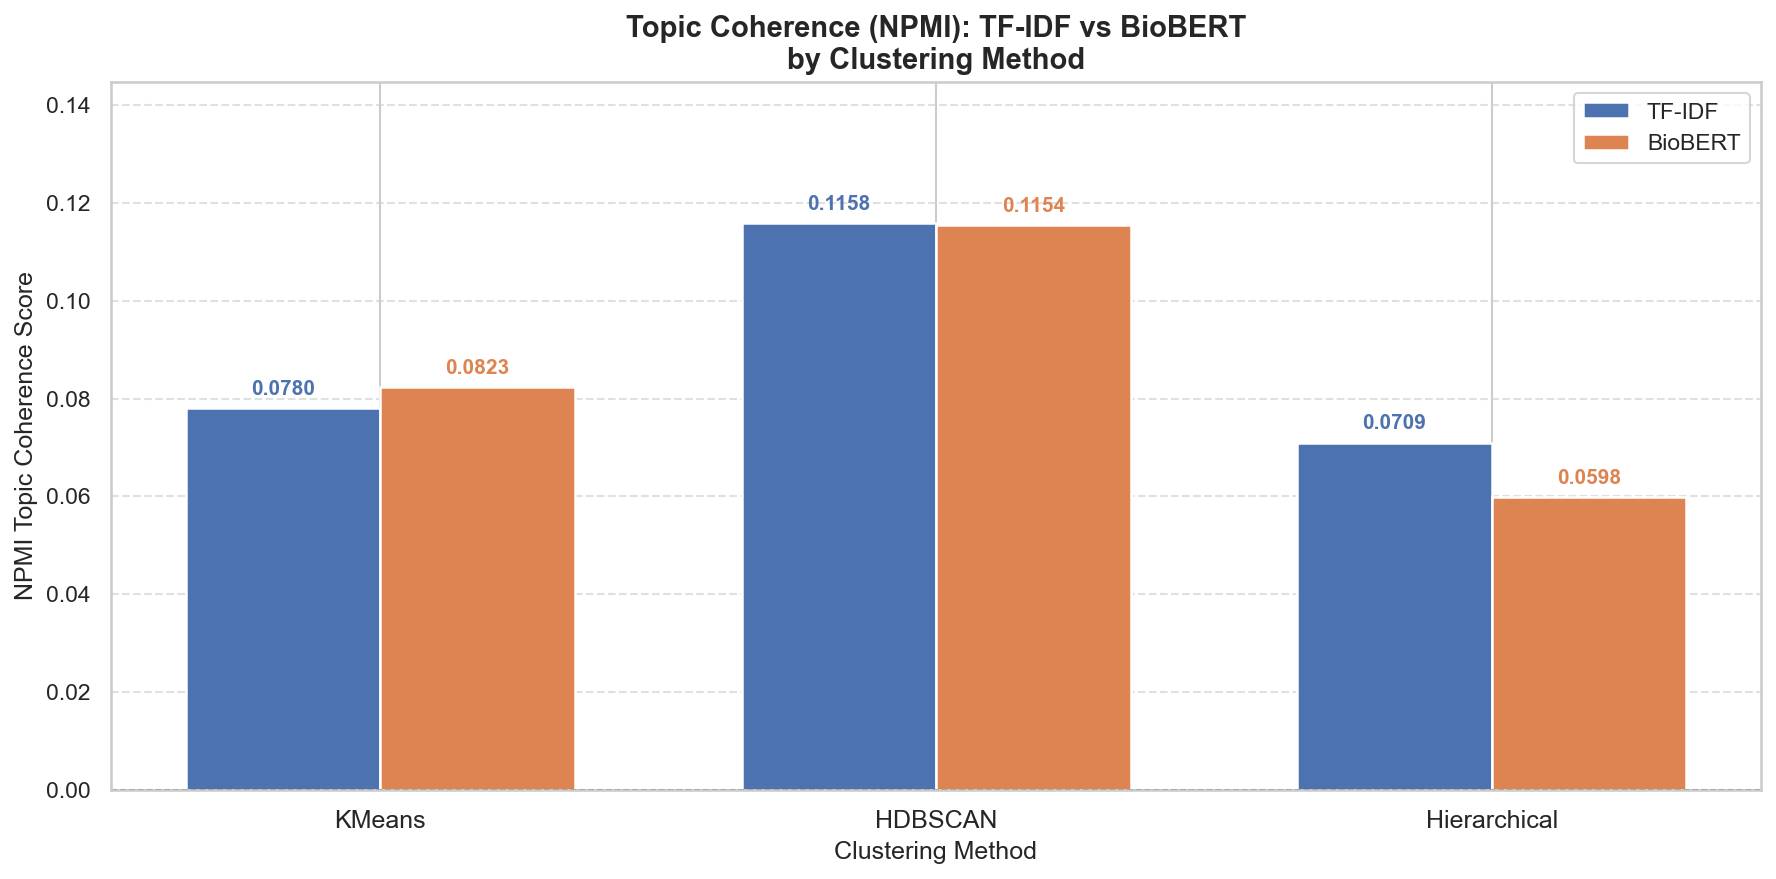
\includegraphics[width=\columnwidth]{Coherence_Results/coherence_grouped_bar.png}
\caption{NPMI topic coherence scores across all six experimental configurations, grouped by clustering algorithm. HDBSCAN achieves the highest coherence under both TF-IDF (0.1158) and BioBERT (0.1154) embeddings, while parametric algorithms (KMeans, Hierarchical) yield substantially lower coherence regardless of the feature extraction strategy.}
\label{fig:eval_metrics}
\end{figure}

\subsection{Macro-Level Clinical Validation}

To assess the clinical interpretability of the clustering results, we examined the five KMeans clusters produced by the BioBERT pipeline. Each cluster was assigned a clinical category by domain experts based on its top TF-IDF keywords. Table~\ref{tab:macro} presents the resulting macro-level disease categories with their corresponding NPMI coherence scores.

\begin{table}[t]
\centering
\caption{Macro-level clinical validation of BioBERT KMeans clusters (K=5). Each cluster is labeled with a clinically meaningful disease category based on its top TF-IDF keywords.}
\label{tab:macro}
\resizebox{\columnwidth}{!}{%
\begin{tabular}{cllc}
\toprule
\textbf{Cluster} & \textbf{Clinical Category} & \textbf{Top Keywords} & \textbf{NPMI} \\
\midrule
0 & Cardiovascular \& Metabolic Risk & patients, risk, care, hypertension, diabetes & 0.0597 \\
1 & Preclinical Molecular Biology   & cells, cell, expression, therapeutic, mice & 0.1092 \\
2 & Oncology \& Case Studies        & clinical, case, treatment, cancer, diagnosis & 0.0797 \\
3 & Clinical Outcomes \& Mortality  & risk, stroke, group, outcomes, mortality & 0.1020 \\
4 & Neurocognitive Disorders        & cognitive, disease, dementia, data, clinical & 0.0611 \\
\bottomrule
\end{tabular}%
}
\end{table}

The five clusters map directly to distinct clinical domains. Cluster~0 captures the intersection of cardiovascular and metabolic diseases (hypertension and diabetes). Cluster~1 represents preclinical molecular biology, dominated by cellular and expression-level research. Cluster~2 corresponds to oncology and clinical case reporting. Cluster~3 focuses on clinical outcomes, mortality, and stroke research. Cluster~4 is specific to neurocognitive disorders, including dementia.

The NPMI coherence values at the macro level range from 0.0597 (Cluster~0) to 0.1092 (Cluster~1). While these values are moderate compared to the micro-level topics discussed below, they represent semantically coherent broad categories that encompass thousands of abstracts each. The variation in coherence reflects the inherent breadth of these categories: clusters covering a wider range of subtopics (e.g., Cardiovascular \& Metabolic Risk) naturally exhibit lower pairwise term co-occurrence than more focused clusters (e.g., Preclinical Molecular Biology).

\subsection{Micro-Level Topic Discovery}

HDBSCAN's density-based approach discovers a much finer-grained topic structure. From the BioBERT pipeline, HDBSCAN identified 80 clusters, of which the top 10 by NPMI coherence are listed in Table~\ref{tab:micro}. These topics reveal highly specific biomedical research themes that are entirely missed at the K=5 macro level.

\begin{table}[t]
\centering
\caption{Micro-level topic discovery: top 10 HDBSCAN clusters from the BioBERT pipeline ranked by NPMI coherence. These topics reveal fine-grained biomedical research themes that are invisible at the K=5 macro level.}
\label{tab:micro}
\resizebox{\columnwidth}{!}{%
\begin{tabular}{cllc}
\toprule
\textbf{Rank} & \textbf{Inferred Topic} & \textbf{Top Keywords} & \textbf{NPMI} \\
\midrule
1  & Ptau Plasma         & ptau, plasma, tau, csf, pet, biomarkers & \textbf{0.3220} \\
2  & Syn Disease         & syn, synuclein, aggregation, tau, amyloid & 0.2822 \\
3  & Cells Cell          & cells, tumor, cancer, immune, therapeutic & 0.2465 \\
4  & Gut Microbiota      & gut, microbiota, microbial, metabolic, axis & 0.2260 \\
5  & Cells Immune        & cells, immune, tumor, immunotherapy, cancer & 0.2183 \\
6  & Disease Mitochondrial & mitochondrial, therapeutic, neurodegenerative, autophagy & 0.1980 \\
7  & Disease Tau         & tau, amyloid, therapeutic, neurodegenerative, pathology & 0.1961 \\
8  & Mice Mitochondrial  & mice, mitochondrial, neuronal, signaling, lipid & 0.1943 \\
9  & Patients Hypertension & hypertension, pressure, blood, kidney, sbp & 0.1829 \\
10 & Disease Mitochondrial & mitochondrial, neurodegenerative, brain, dysfunction & 0.1819 \\
\bottomrule
\end{tabular}%
}
\end{table}

The top micro-level topics achieve NPMI coherence values substantially higher than any macro-level cluster. Ptau Plasma (rank~1, NPMI~0.322) and Syn Disease (rank~2, NPMI~0.282) represent highly specialized biomarker research themes with tight term co-occurrence. The Gut Microbiota topic (rank~4, NPMI~0.226) captures a distinct interdisciplinary research area spanning metabolic and neurological disease.

Several observations support the validity of these micro-topics. First, the topics are domain-specific and immediately interpretable: a researcher familiar with biomedical literature can identify the research focus of each cluster from its top keywords alone. Second, topics that might be expected to merge at coarser granularity (e.g., two distinct mitochondrial disease topics at ranks~6 and~10) are correctly separated by HDBSCAN, preserving nuanced distinctions. Third, the NPMI coherence gradient from rank~1 (0.322) to rank~10 (0.182) is smooth, suggesting that the coherence measure captures meaningful variation in topic thematic specificity rather than arbitrary noise.

Fig.~\ref{fig:coherence_comparison} compares the NPMI coherence distribution of the top 10 HDBSCAN micro-topics against the average coherence of the five KMeans macro categories. The micro-level topics substantially exceed the macro-level baseline, demonstrating that density-based clustering at the appropriate granularity reveals topic structures with significantly higher semantic coherence.

\begin{figure}[t]
\centering
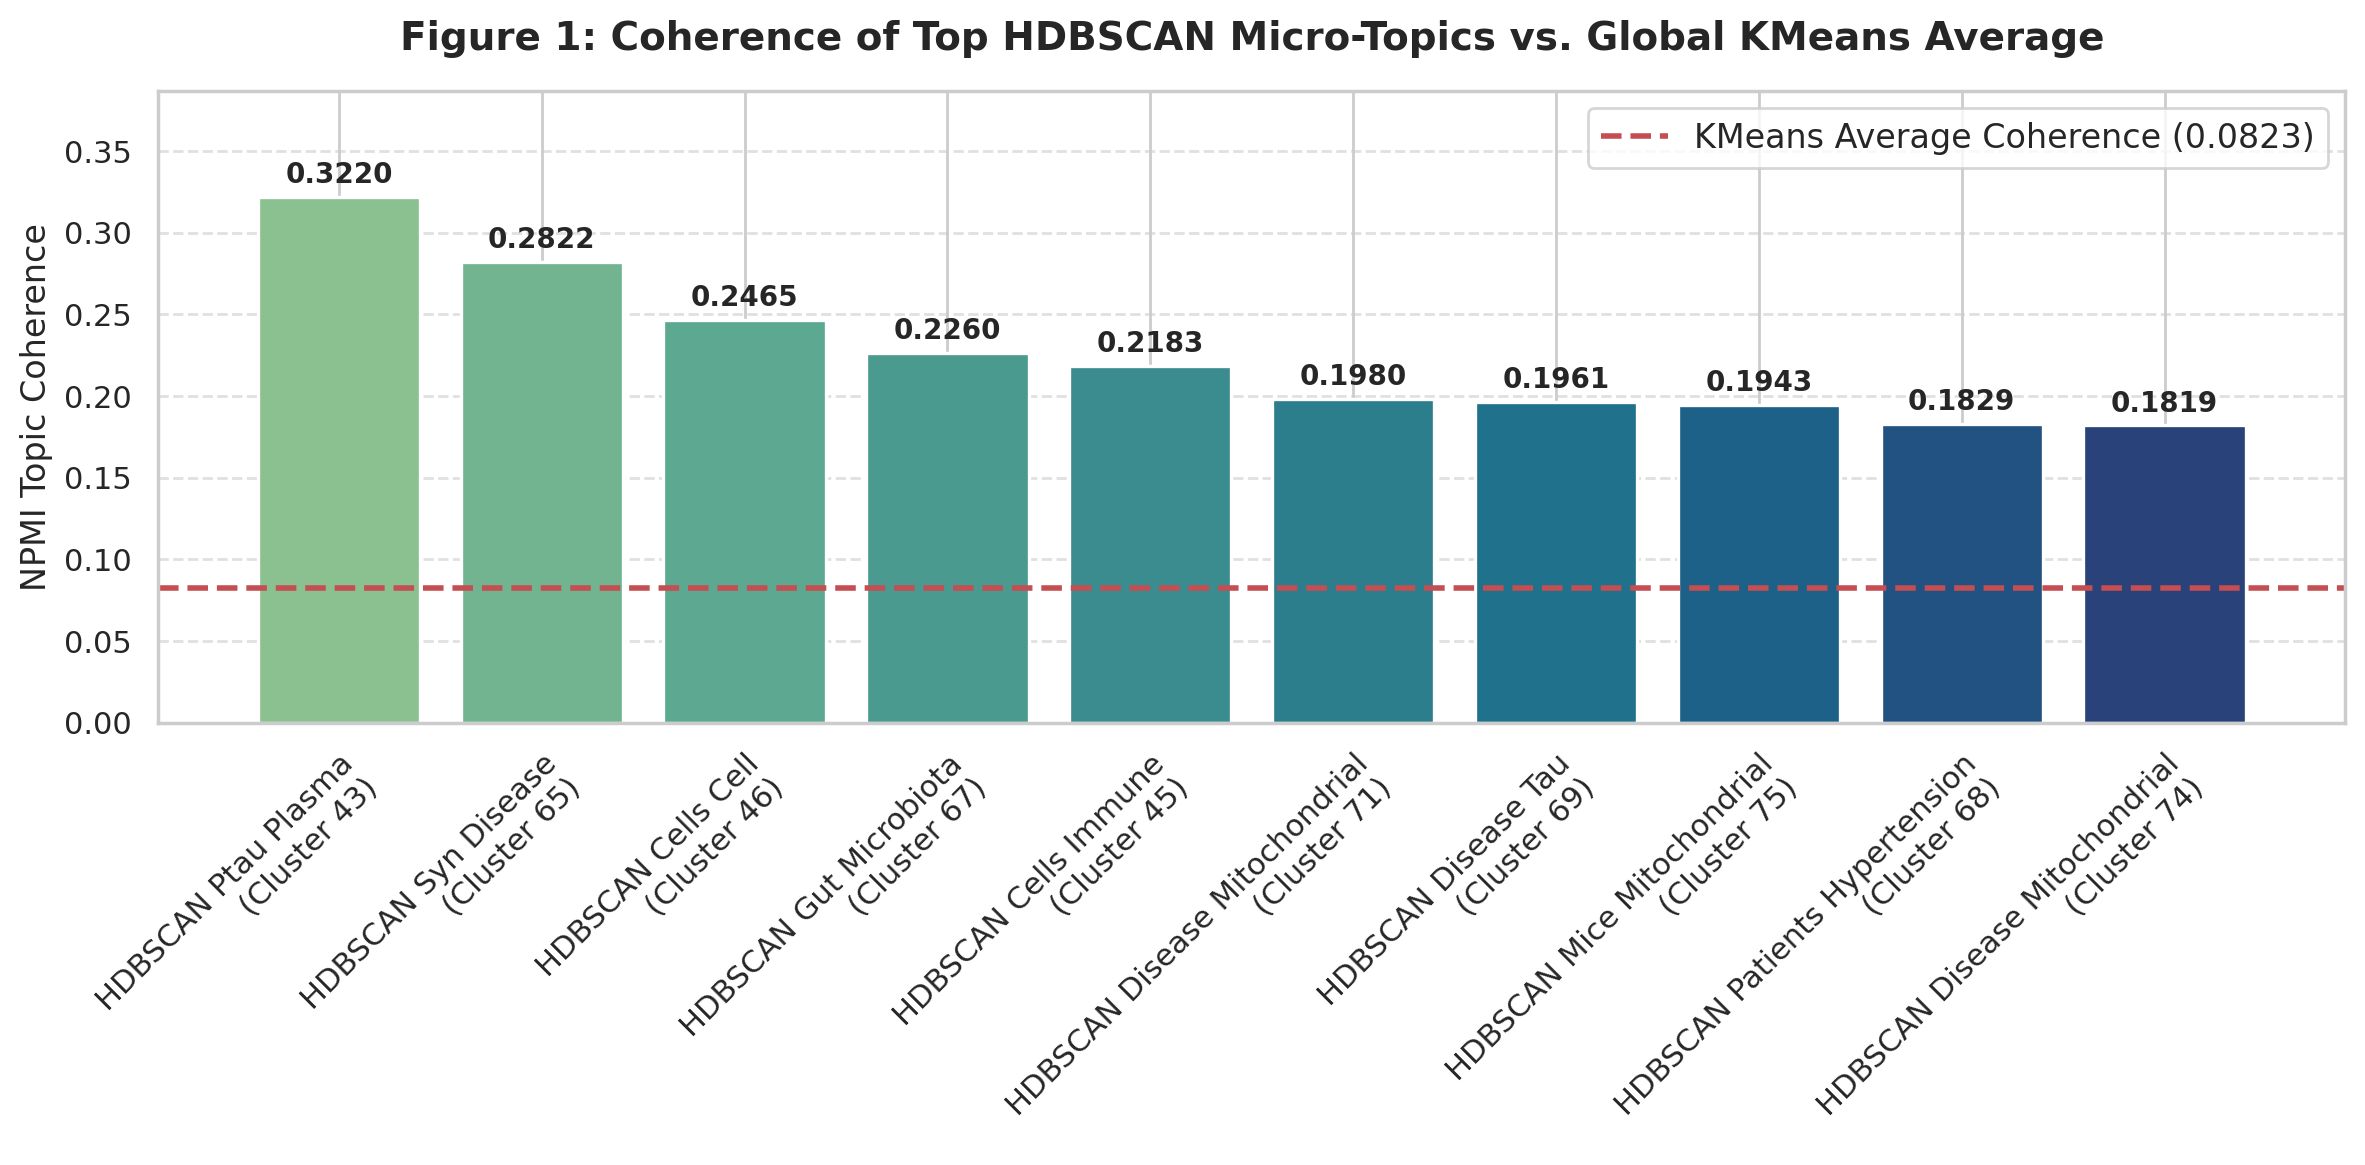
\includegraphics[width=\columnwidth]{Manuscript_Results/Figure1_HDBSCAN_vs_KMeans_Coherence.png}
\caption{Comparison of NPMI coherence between the top 10 HDBSCAN micro-topics and the average KMeans macro-level coherence (dashed red line). HDBSCAN topics achieve substantially higher coherence, with the top topic (Ptau Plasma, NPMI~0.322) exceeding the KMeans average by a factor of approximately four.}
\label{fig:coherence_comparison}
\end{figure}

\subsection{Disease Knowledge Map Visualization}

The final UMAP projections with automated disease labels (Fig.~\ref{fig:knowledge_maps}) provide a qualitative view of how each clustering algorithm organizes the biomedical embedding space. The KMeans panel shows five broad, well-separated regions corresponding to the clinical categories in Table~\ref{tab:macro}. The HDBSCAN panel reveals a more complex topology with numerous small clusters and a substantial noise region (gray points), reflecting the genuine heterogeneity of biomedical research themes. The hierarchical clustering panel produces a partition that is intermediate in visual structure between the two.

\begin{figure}[t]
\centering
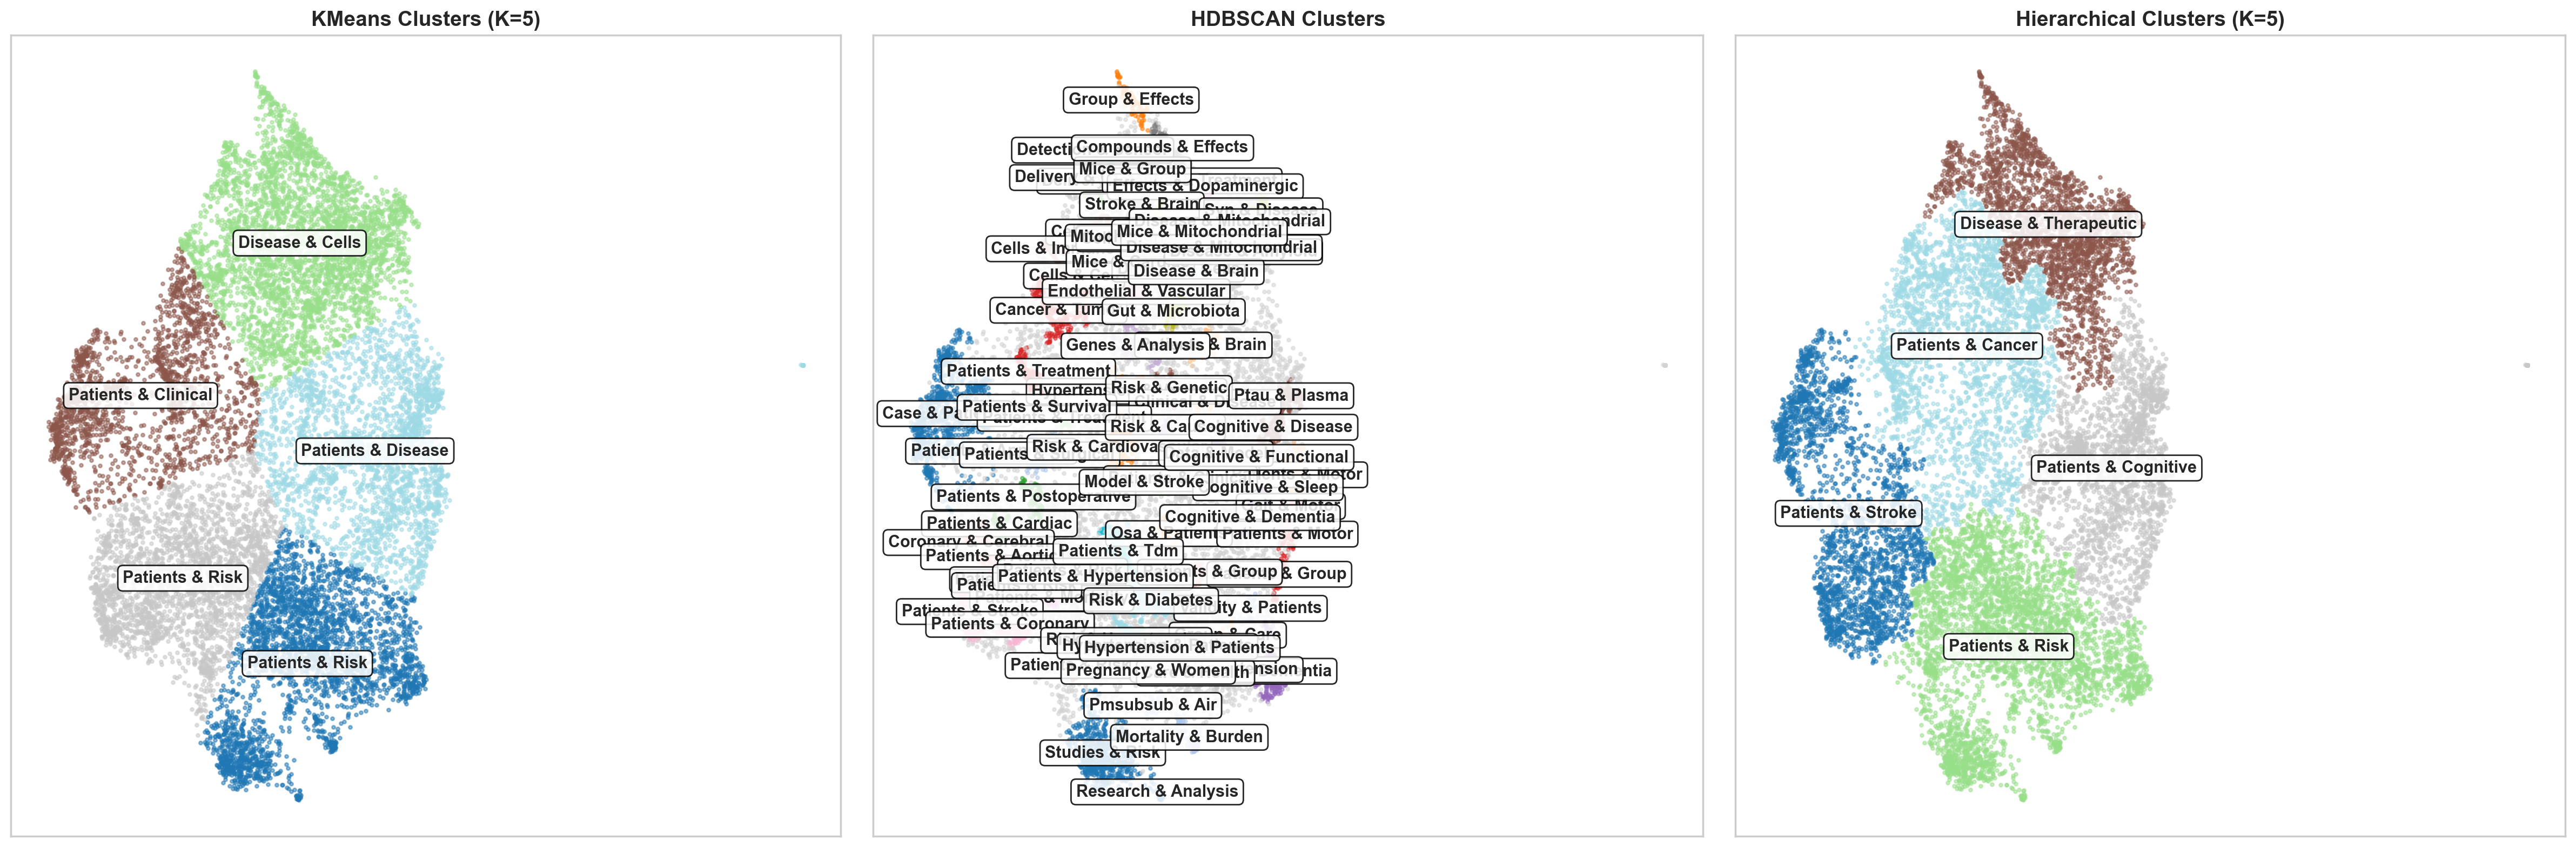
\includegraphics[width=\columnwidth]{BioBERT_Results/step11_final_mapped_umap_all_algorithms.png}
\caption{Final UMAP 2D projections of BioBERT embeddings with automated disease labels for KMeans (left), HDBSCAN (center), and hierarchical clustering (right). HDBSCAN reveals a rich substructure of 80 fine-grained topics that is entirely invisible in the KMeans and hierarchical solutions. Gray points in the HDBSCAN panel represent noise points (label --1) that the algorithm correctly identifies as not belonging to any dense cluster.}
\label{fig:knowledge_maps}
\end{figure}

\section{Discussion}

The experimental results presented in Section~IV yield three principal findings with implications for unsupervised disease knowledge mapping from biomedical text. First, the choice of clustering algorithm has a substantially larger impact on clustering quality and topic coherence than the choice of embedding method. Second, density-based clustering with HDBSCAN discovers an order of magnitude more topics than parametric alternatives, and these topics are both more coherent and more interpretable. Third, TF-IDF frequency features and BioBERT contextual embeddings produce comparable topic coherence when paired with HDBSCAN, challenging the assumption that deeper representations are always necessary for unsupervised biomedical text organization.

\subsection{The Primacy of Clustering Algorithm over Embedding Method}

Across all three evaluation metrics, the variance attributable to the clustering algorithm exceeds the variance attributable to the embedding strategy. HDBSCAN achieves the highest scores in both pipelines on every metric, and the performance gap between HDBSCAN and the next-best algorithm is consistently larger than the gap between TF-IDF and BioBERT for any fixed algorithm. This finding has practical significance: researchers building unsupervised biomedical document organization systems should prioritize the flexibility of the clustering component over the sophistication of the embedding step.

The explanation lies in the distributional properties of biomedical embedding spaces. Biomedical research themes do not follow the spherical, equal-sized distribution that KMeans implicitly assumes, nor the balanced hierarchical structure that Ward linkage expects. Density-based clustering, by contrast, accommodates arbitrarily shaped clusters of varying sizes and densities, which is precisely the structure that real biomedical topic spaces exhibit. Davagdorj et al.~\cite{ref15} observed that BioBERT-GMM outperformed KMeans and agglomerative clustering on PubMed abstracts, but GMM still assumes Gaussian cluster shapes and requires a fixed $K$. Our results extend their finding by showing that removing both the parametric shape assumption and the fixed-$K$ requirement yields further substantial improvements.

\subsection{Implications for Embedding Selection in Biomedical NLP}

The near-identical NPMI coherence of TF-IDF+HDBSCAN (0.1158) and BioBERT+HDBSCAN (0.1154) is a noteworthy result. It suggests that for the task of organizing documents into topically coherent groups, the discriminative signal carried by term frequency distributions is largely redundant with the semantic signal captured by contextual embeddings. This is consistent with the observation that cluster-level TF-IDF keyword extraction (c-TF-IDF) is the mechanism by which BERTopic~\cite{ref17} achieves its topic quality, regardless of the underlying embedding model.

However, this equivalence does not hold under restrictive clustering algorithms. BioBERT+KMeans (Silhouette 0.4112) substantially outperforms TF-IDF+KMeans (Silhouette 0.3708), demonstrating that richer embeddings compensate for algorithmic inflexibility. The practical implication is that biomedical NLP researchers should consider the full pipeline: a simple embedding with a flexible clustering algorithm can match a complex embedding with a restrictive one, but the reverse is not true.

The BioBERT embedding generation required approximately 35 minutes of CPU time for 14,064 abstracts versus seconds for TF-IDF. For resource-constrained settings, TF-IDF+HDBSCAN offers a cost-effective alternative that sacrifices no topic coherence quality. When deeper cluster interpretability is desired, BioBERT embeddings enable the macro-level clinical validation (Table~\ref{tab:macro}) that shows cleaner alignment with known disease categories.

\subsection{Macro and Micro Interpretability}

A strength of our pipeline design is its ability to produce interpretable results at two distinct granularity levels. The macro level (KMeans, $K=5$) yields broad clinical categories that correspond to recognized disease groupings: cardiovascular and metabolic risk, preclinical molecular biology, oncology, clinical outcomes, and neurocognitive disorders. These categories provide an accessible high-level map of the research landscape that could assist literature reviewers in understanding the thematic composition of a disease corpus.

The micro level (HDBSCAN, 80--116 topics) captures the genuine thematic heterogeneity of biomedical research. The top-10 topics by NPMI coherence include highly specific themes such as Ptau Plasma biomarkers for Alzheimer's disease (NPMI 0.322), alpha-synuclein aggregation pathways in Parkinson's disease (NPMI 0.282), and gut microbiota research spanning metabolic and neurological disciplines (NPMI 0.226). These topics are not merely statistically coherent but also clinically meaningful: Ptau plasma has emerged as a leading blood-based biomarker candidate for Alzheimer's disease, and the alpha-synuclein aggregation pathway is a central focus of Parkinson's disease research. The fact that our fully unsupervised pipeline surfaces these topics without any labeled data or domain-specific tuning demonstrates the power of combining domain-adapted embeddings with density-based clustering.

The two-level structure also addresses a known limitation of HDBSCAN: it can produce a very large number of clusters, some of which may be too specific to be useful for high-level summarization. By complementing HDBSCAN's micro-topics with KMeans macro-categories, our pipeline provides both the broad overview needed for executive understanding and the fine-grained detail needed for specialized literature exploration.

\subsection{Comparison with Existing Frameworks}

Our pipeline shares architectural similarities with BERTopic~\cite{ref17}, which also uses HDBSCAN clustering with cluster-level TF-IDF (c-TF-IDF) for topic labeling. Two differences are consequential. First, BERTopic uses general-domain sentence-transformer models, whereas our BioBERT configuration uses a model specifically pretrained on biomedical text, which has been shown to capture relational knowledge between biomedical concepts more accurately~\cite{ref20}. Second, our systematic six-configuration comparison provides evidence about which pipeline components drive performance, rather than evaluating a single configuration.

The LORE framework~\cite{ref11} demonstrated that UMAP projections of disease-gene embeddings exhibit geometric structure with biological meaning, a finding that our results corroborate and extend to the document level. While LORE targets gene-disease association prediction with 90\% mean average precision, our pipeline targets corpus-level thematic discovery, a complementary task that existing literature mining systems have not addressed. Knowledge graph approaches~\cite{ref8}~\cite{ref9}~\cite{ref10} organize information around predefined entity types and relations, making them suitable for structured querying but not for discovering the emergent thematic structure of a document corpus.

\subsection{Limitations and Future Work}

Several limitations of this study should be acknowledged. First, clustering was performed on UMAP 2D projections rather than on the original high-dimensional feature spaces. While UMAP preserves local and global structure, information loss is inevitable in the reduction from 5,000 or 768 dimensions to two. Future work should evaluate whether clustering the original embeddings yields different topic structures, particularly for BioBERT where the 768-dimensional space may retain fine-grained distinctions that UMAP projection smooths over.

Second, the Elbow method for determining optimal $K$ for KMeans and hierarchical clustering operates on the UMAP embedding space and may reflect the dimensionality reduction rather than the true data structure. Alternative $K$ selection methods (silhouette analysis, gap statistic, stability-based approaches) could yield different macro-level partitions and should be investigated.

Third, the BioBERT embedding extraction used a maximum sequence length of 128 tokens. While this covers most PubMed abstracts, longer abstracts are truncated, potentially losing information relevant to fine-grained topic discrimination. Increasing the sequence length or employing hierarchical document representations could improve topic quality for longer documents.

Fourth, the dataset is limited to English-language PubMed abstracts from eight disease queries. The generalizability of our findings to full-text articles, non-English biomedical literature, clinical notes, or other scientific domains (genomics, proteomics, drug discovery) remains to be tested.

Fifth, the NPMI coherence metric measures term co-occurrence within the corpus itself, which is an intrinsic rather than extrinsic evaluation. While high NPMI has been shown to correlate with human judgment of topic quality, future work should include expert annotation of topic interpretability and clinical relevance for a subset of clusters.

Sixth, the R implementation (Appendix~A) demonstrates the pipeline's language-agnostic design using a different set of parameters (K=8, minPts=50}), achieving qualitatively similar results. This cross-language reproducibility strengthens confidence in the approach's robustness.

Finally, the pipeline currently treats each document independently. Incorporating citation networks, author affiliation metadata, or temporal trends could enrich the knowledge maps with relational and longitudinal dimensions. Extending the pipeline to track how disease research themes evolve over time is a natural direction for future work.

\subsection{Summary of Contributions}

This study demonstrates that an unsupervised pipeline combining TF-IDF or BioBERT feature extraction with UMAP dimensionality reduction and HDBSCAN density-based clustering can automatically discover clinically meaningful disease research themes from PubMed abstracts without any labeled training data. The modular pipeline design allows researchers to select the feature extraction and clustering components best suited to their computational resources and interpretability requirements. The systematic six-configuration comparison provides evidence-based guidance for pipeline design in biomedical text analysis. All code, output files, and detailed documentation are publicly available to support reproducibility and further development.

\section{Conclusion}

This paper presented a systematic comparison of six unsupervised configurations for disease knowledge mapping from PubMed abstracts, crossing two feature extraction methods (TF-IDF and BioBERT) with three clustering algorithms (KMeans, HDBSCAN, and hierarchical clustering). The evaluation across 14,064 biomedical abstracts from eight disease categories, using Silhouette coefficient, Davies--Bouldin index, and NPMI topic coherence, produced three main findings.

First, HDBSCAN consistently outperformed both parametric alternatives, achieving the highest Silhouette (0.4786 for TF-IDF, 0.4225 for BioBERT), lowest Davies--Bouldin (0.6034 for TF-IDF, 0.7068 for BioBERT), and highest NPMI coherence (0.1158 for TF-IDF, 0.1154 for BioBERT). Density-based clustering discovered 116 topics (TF-IDF) and 80 topics (BioBERT), compared to the fixed five topics produced by the Elbow-constrained KMeans and hierarchical approaches.

Second, TF-IDF with HDBSCAN matched BioBERT with HDBSCAN on topic coherence, demonstrating that frequency-based features remain highly competitive with contextual embeddings when paired with a sufficiently flexible clustering algorithm. The practical implication is that high-quality unsupervised topic discovery from biomedical text does not necessarily require deep transformer models, making the approach accessible in resource-constrained settings.

Third, the two-level interpretability framework, combining macro-level KMeans clinical categories (Cardiovascular \& Metabolic Risk, Preclinical Molecular Biology, Oncology \& Case Studies, Clinical Outcomes \& Mortality, Neurocognitive Disorders) with micro-level HDBSCAN topics (e.g., Ptau Plasma at NPMI 0.322, Syn Disease at 0.282, Gut Microbiota at 0.226), provides a comprehensive view of disease research structure at both broad and granular scales.

The modular pipeline is language-agnostic; an independent R implementation with different parameter choices (K=8, minPts=50}) produced qualitatively consistent knowledge maps, supporting cross-language reproducibility.

Future work should extend the pipeline to full-text articles, incorporate temporal dynamics to track the evolution of disease research themes, integrate structured metadata (citation networks, funding data), and evaluate topic quality through expert clinical annotation. The growing volume of biomedical literature makes unsupervised knowledge discovery tools increasingly essential for research synthesis, and density-based clustering with appropriate feature representations offers a scalable and effective path forward.

\begin{thebibliography}{00}
\bibitem{ref1} J. Lee, W. Yoon, S. Kim, D. Kim, S. Kim, C. H. So, and J. Kang, ``BioBERT: a pre-trained biomedical language representation model for biomedical text mining,'' \textit{Bioinformatics}, vol.~36, no.~4, pp.~1234--1240, Feb.~2020, doi: 10.1093/bioinformatics/btz682.

\bibitem{ref2} S. Kumar and T. Basu, ``AdaBioBERT: adaptive token sequence learning for biomedical named entity recognition,'' in \textit{Proc. 24th Workshop Biomed. Lang. Process. (BioNLP 2025)}, Bangkok, Thailand, Aug.~2025, pp.~56--62.

\bibitem{ref3} Y. Peng, S. Yan, and Z. Lu, ``Transfer learning in biomedical natural language processing: an evaluation of BERT and ELMo on ten benchmarking datasets,'' in \textit{Proc. BioNLP 2019 Workshop}, Florence, Italy, Aug.~2019, pp.~58--65.

\bibitem{ref4} Y. Peng, Q. Chen, and Z. Lu, ``An empirical study of multi-task learning on BERT for biomedical text mining,'' in \textit{Proc. BioNLP 2020 Workshop}, Online, Jul.~2020, pp.~205--214.

\bibitem{ref5} S. Alrowili and K. Vijay-Shanker, ``BioM-Transformers: building large biomedical language models with BERT, ALBERT and ELECTRA,'' in \textit{Proc. BioNLP 2021 Workshop}, Online, Jun.~2021, pp.~221--227.

\bibitem{ref6} D. Vithanage, P. Yu, L. Wang, and C. Deng, ``Contextual word embedding for biomedical knowledge extraction: a rapid review and case study,'' \textit{J. Healthcare Inform. Res.}, vol.~8, no.~1, pp.~158--179, Jan.~2024, doi: 10.1007/s41666-023-00157-y.

\bibitem{ref7} S. Sharaf and V. S. Anoop, ``An analysis on large language models in healthcare: a case study of BioBERT,'' arXiv:2310.07282 [cs.AI], Oct.~2023.

\bibitem{ref8} D. Grissa, A. Junge, T. I. Oprea, and L. J. Jensen, ``DISEASES 2.0: a weekly updated database of disease--gene associations from text mining and data integration,'' \textit{Database}, vol.~2022, Art. no.~baac019, Mar.~2022, doi: 10.1093/database/baac019.

\bibitem{ref9} J. Xu, S. Kim, M. Song, M. Jeong, D. Kim, J. Kang, \textit{et al.}, ``Building a PubMed knowledge graph,'' \textit{Sci. Data}, vol.~7, no.~1, Art. no.~205, Jun.~2020, doi: 10.1038/s41597-020-0543-2.

\bibitem{ref10} A. D. Diaz Gonzalez, S. Yue, S. T. Hayes, and K. S. Hughes, ``Applying BioBERT to extract germline gene-disease associations for building a knowledge graph from the biomedical literature,'' in \textit{Proc. 7th Int. Conf. Inf. Syst. Data Mining (ICISDM '23)}, Atlanta, GA, USA, May~2023, 6 pages, doi: 10.1145/3603765.3603771.

\bibitem{ref11} P.-H. Li, Y.-Y. Sun, H.-F. Juan, and C.-Y. Chen, ``A large language model framework for literature-based disease--gene association prediction,'' \textit{Briefings Bioinform.}, vol.~26, no.~1, Art. no.~bbaf070, Feb.~2025, doi: 10.1093/bib/bbaf070.

\bibitem{ref12} Z. Zhang, N. Parulian, H. Ji, A. S. Elsayed, S. Myers, and M. Palmer, ``Fine-grained information extraction from biomedical literature based on knowledge-enriched abstract meaning representation,'' in \textit{Proc. 59th Annu. Meeting Assoc. Comput. Linguist. 11th Int. Joint Conf. Nat. Lang. Process. (ACL-IJCNLP 2021)}, Online, Aug.~2021, pp.~6261--6270.

\bibitem{ref13} S. Masoumi, H. Amirkhani, N. Sadeghian, and S. Shahraz, ``Natural language processing (NLP) to facilitate abstract review in medical research: the application of BioBERT to exploring the 20-year use of NLP in medical research,'' \textit{Syst. Rev.}, vol.~13, no.~1, Art. no.~107, 2024, doi: 10.1186/s13643-024-02470-y.

\bibitem{ref14} Y.-N. Chuang, G. Wang, C.-Y. Chang, K.-H. Lai, D. Zha, R. Tang, \textit{et al.}, ``DiscoverPath: a knowledge refinement and retrieval system for interdisciplinarity on biomedical research,'' in \textit{Proc. 32nd ACM Int. Conf. Inf. Knowl. Manage. (CIKM '23)}, Birmingham, U.K., Oct.~2023, 5 pages, doi: 10.1145/3583780.3614739.

\bibitem{ref15} K. Davagdorj, L. Wang, M. Li, V.-H. Pham, K. H. Ryu, and N. Theera-Umpon, ``Discovering thematically coherent biomedical documents using contextualized bidirectional encoder representations from transformers-based clustering,'' \textit{Int. J. Environ. Res. Public Health}, vol.~19, no.~10, Art. no.~5893, May~2022, doi: 10.3390/ijerph19105893.

\bibitem{ref16} N. M. AbdelAziz, A. A. Ali, S. M. Naguib, and L. S. Fayed, ``Clustering-based topic modeling for biomedical documents extractive text summarization,'' \textit{J. Supercomput.}, vol.~81, no.~1, Art. no.~171, 2025, doi: 10.1007/s11227-024-06640-6.

\bibitem{ref17} M. Grootendorst, ``BERTopic: neural topic modeling with a class-based TF-IDF procedure,'' arXiv:2203.05794 [cs.CL], Mar.~2022.

\bibitem{ref18} A. Munoz-Farre, A. Poulakakis-Daktylidis, D. M. Kothalawala, and A. Rodriguez-Martinez, ``Interpreting deep embeddings for disease progression clustering,'' arXiv:2307.06060 [stat.ML], Jul.~2023.

\bibitem{ref19} N. Oubenali, S. Messaoud, A. Filiot, A. Lamer, and P. Andrey, ``Visualization of medical concepts represented using word embeddings: a scoping review,'' \textit{BMC Med. Inform. Decis. Mak.}, vol.~22, no.~1, Art. no.~83, Mar.~2022, doi: 10.1186/s12911-022-01822-9.

\bibitem{ref20} S. S. Panesar, ``Biomedical knowledge discovery from unstructured text corpora using contextual word embeddings,'' Research Square, preprint, Nov.~2022, doi: 10.21203/rs.3.rs-2286334/v1.

\end{thebibliography}

\end{document}
